\documentclass[a4paper]{scrreprt}
\usepackage{graphicx}
\usepackage{graphics}

\begin{document}
\chapter{Your Chapter}
Lorem ipsum dolor sit amet, consetetur sadipscing elitr, sed diam
nonumy eirmod tempor invidunt ut labore et dolore magna aliquyam
erat, sed diam voluptua. At vero eos et accusam et justo duo dolores
et ea
rebum. Stet clita kasd gubergren, no sea takimata sanctus est Lorem
ipsum dolor sit amet. Lorem ipsum dolor sit amet, consetetur
sadipscing elitr, sed diam nonumy eirmod tempor invidunt ut labore et
dolore magna aliquyam erat, sed diam voluptua. At vero eos et accusam
et justo duo dolores et ea rebum. Stet clita kasd gubergren, no sea
takimata sanctus est Lorem ipsum dolor sit amet.

\begin{figure}[ht]
    \begin{minipage}[b]{0.45\linewidth}
        \centering
        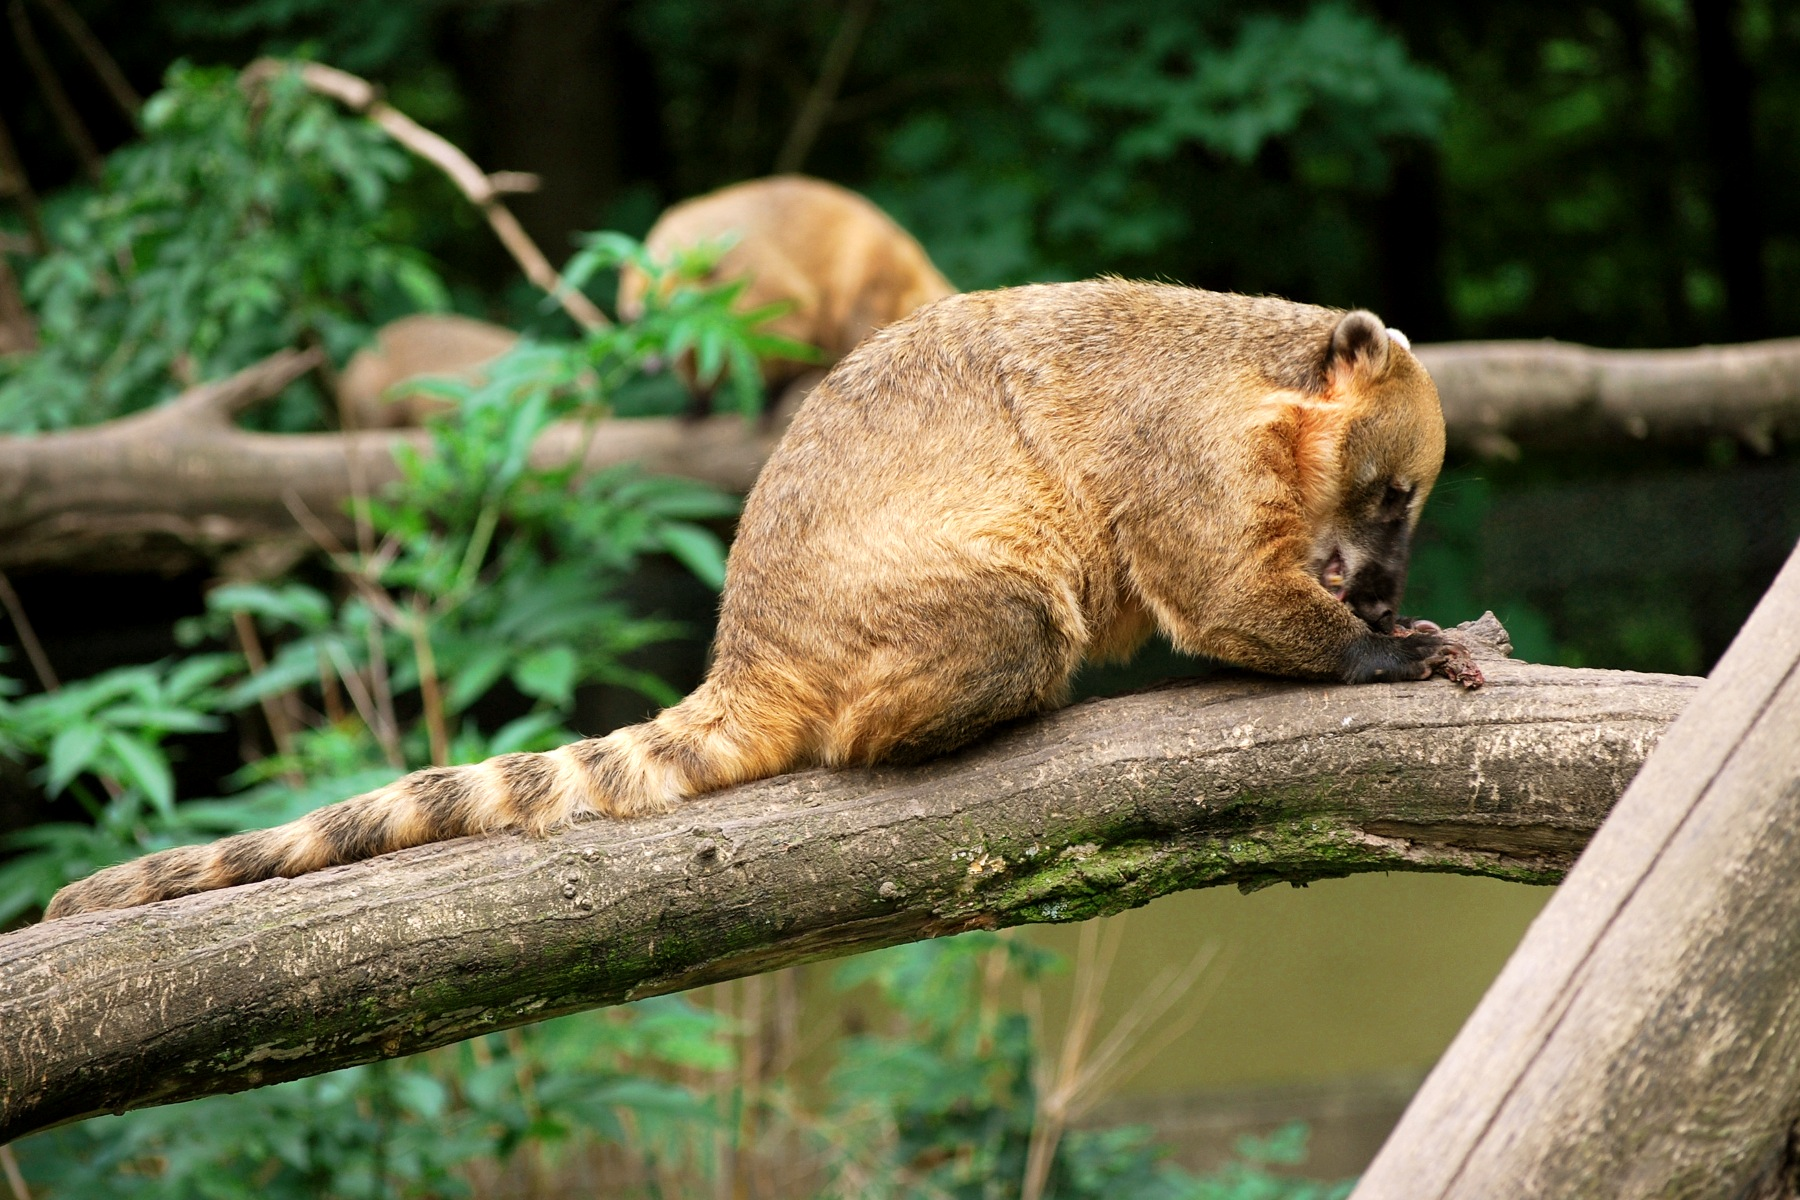
\includegraphics[width=\textwidth]{YourImage.jpg}
        \caption{South American coati}
        \label{fig:nasua}
    \end{minipage}
    \hspace{0.5cm}
    \begin{minipage}[b]{0.45\linewidth}
        \centering
        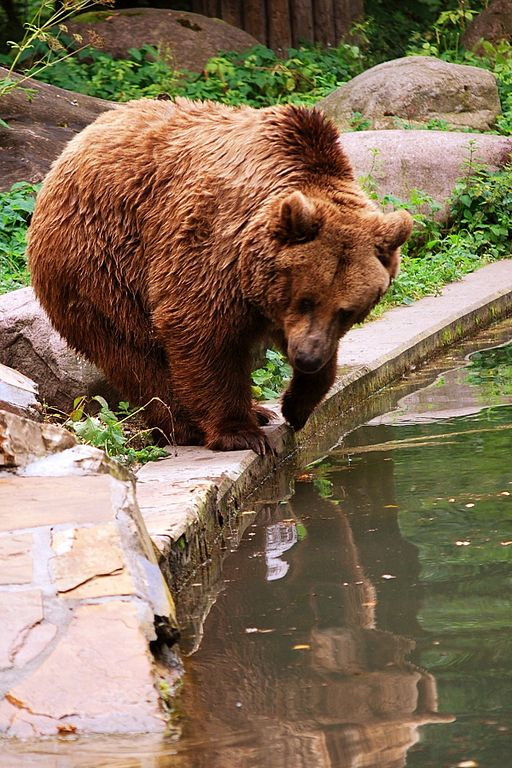
\includegraphics[width=\textwidth]{Ursus-arctos.jpg}
        \caption{Brown bear}
        \label{fig:Ursus-arctos}
    \end{minipage}
\end{figure}

You can now see that a Nasua nasua in figure \ref{fig:nasua} and a Ursus-arctos
in figure \ref{fig:Ursus-arctos}. Note that you have to run LaTeX twice and
don't delete intermediate files when you want to use ref.

\end{document}
